\documentclass{report}

\usepackage{preamble}
\usepackage{prealgebra}
\usepackage{premath}
\usepackage{precomb}

\usepackage{biblatex}
\addbibresource{report.bib}

% Remove "chapter" heading
\usepackage{titlesec}
\titleformat{\chapter}{\normalfont\huge\bf}{\thechapter.}{20pt}{\huge\bf}

\newcommand*{\vertbar}{\rule[-1ex]{0.5pt}{2.5ex}}
\newcommand*{\horzbar}{\rule[.5ex]{2.5ex}{0.5pt}}
\newcommand{\mysep}{
  \begin{center}
  \scalebox{0.2}{
  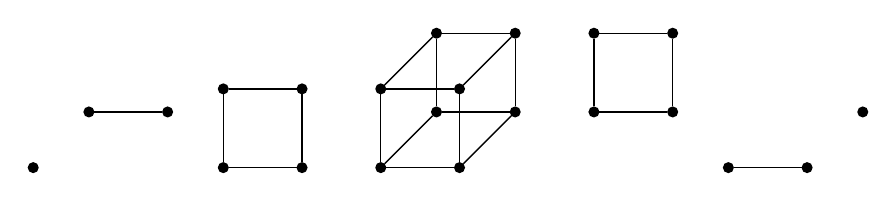
\begin{tikzpicture}
    \tikzset{
      dot/.style = {circle, fill, minimum size=4pt,
      inner sep=0pt, outer sep=0pt},
      dot/.default = 4pt % size of the circle diameter
    }

    \node[dot] (-) {};

    \node[dot, above right of = -] (0) {};
    \node[dot, right of = 0] (1) {};
    \draw (0) edge (1);

    \node[dot, below right of = 1] (00) {};
    \node[dot, right of = 00] (01) {};
    \node[dot, above of = 00] (10) {};
    \node[dot, right of = 10] (11) {};
    \draw[-, line width=0.5pt]
      (00) edge (01)
      (00) edge (10)
      (01) edge (11)
      (10) edge (11)
    ;

    \node[dot, right of = 01] (000) {};
    \node[dot, right of = 000] (001) {};
    \node[dot, above of = 000] (010) {};
    \node[dot, right of = 010] (011) {};
    \node[dot, above right of = 000] (100) {};
    \node[dot, right of = 100] (101) {};
    \node[dot, above of = 100] (110) {};
    \node[dot, right of = 110] (111) {};
    \draw[-, line width=0.5pt]
      (001) edge (101)
      (010) edge (011)
      (010) edge (110)
      (000) edge (001)
      (001) edge (011)
      (101) edge (111)
      (100) edge (101)
      (100) edge (110)
      (000) edge (010)
      (000) edge (100)
      (110) edge (111)
      (011) edge (111)
    ;

    \node[dot, right of = 101] (00') {};
    \node[dot, right of = 00'] (01') {};
    \node[dot, above of = 00'] (10') {};
    \node[dot, right of = 10'] (11') {};
    \draw[-, line width=0.5pt]
      (00') edge (01')
      (00') edge (10')
      (01') edge (11')
      (10') edge (11')
    ;

    \node[dot, below right of = 01'] (0') {};
    \node[dot, right of = 0'] (1') {};
    \draw (0') edge (1');

    \node[dot, above right of = 1'] (-') {};
  \end{tikzpicture}
  }
  \end{center}
}

\usepackage{array}
\newcolumntype{C}{>{$\displaystyle}c<{$}}  % math display mode in table
% A new columntype to apply automatic stepping
\newcounter{rowcntr}[table]
\renewcommand{\therowcntr}{\thetable.\arabic{rowcntr}}
\newcolumntype{N}{>{\refstepcounter{rowcntr}\therowcntr}c}
\AtBeginEnvironment{tabular}{\setcounter{rowcntr}{0}}  % reset the rowcntr counter at each new tabular

\newcommand{\AS}{\mathcal{A}}
\newcommand{\BMA}{\mathbb{A}}
\newcommand{\Zq}{\Z_q}
\newcommand{\Zqz}{\Z_q \setminus \set{0}}
\newcommand{\Zqd}{\Z_q^d}
\newcommand{\diag}[1]{\operatorname{diag}\( #1 \)}
\newcommand{\chiN}{\chi_{N}}
\newcommand{\chiM}{\chi_{M}}
\newcommand{\chiNs}{\chi_{N^*}}
\newcommand{\chiMs}{\chi_{M^*}}
\newcommand{\diagz}{\diag{\chi_0}}
\newcommand{\diagN}{\diag{\chiN}}
\newcommand{\diagM}{\diag{\chiM}}
\newcommand{\diagNs}{\diag{\chiNs}}
\newcommand{\diagMs}{\diag{\chiMs}}
\newcommand{\diagnu}{\diag{\nu}}
\newcommand{\diagmu}{\diag{\mu}}
\newcommand{\vone}{\mathbf{1}}

\title{Cliques in Association Schemes}
\author{
  Andrew Nagarajah \\
  Supervised by: Prof. Mike Newman
}
\date{\today}

\begin{document}

\maketitle

\begin{abstract}

  This report is an exploration of some of the topics within \emph{Delsarte
  theory}, which uses ideas from graph theory, algebra, and optimization to
  address questions in coding theory in particular, and combinatorics more
  broadly.  The centre of study is the \emph{association scheme}, which provides
  a setting in which to view various objects, especially \emph{distance-regular
  graphs}.  This perspective enables the computation of various parameters of
  interest, including the eigenvalues of graphs and upper bounds on codes,
  cliques, and independent sets.

  This report aims to be mostly self-contained, though background knowledge of
  basic linear algebra and group theory is required.  The important aspects of
  this theory is reviewed in the appendix.

\end{abstract}

\tableofcontents

\chapter{Introduction}
  \section{Coding Theory}
    I'm also not sure if I should include a section like this, but seeing as
    coding theory was the original motivation behind Delsarte's LP bound,
    and it remains (presumably?) a strong motivator for this theory,
    I figured it might be interesting to mention this as an application.

    \begin{itemize}
      \item Basics of Coding Theory
      \item Linear Graphs
      \item Finite Vector Spaces
    \end{itemize}

  \section{Hamming Graphs}

  \section{Distance-Regular Graphs}
    Define $M$-cliques.

    I'm not sure if I should maybe merge this section with $P$-polynomial
    section?

    \begin{itemize}
      \item Definition
      \item Basic parameters
      \item Examples?
    \end{itemize}

\chapter{Association Schemes}
  \section{Association Schemes}\label{sec:AS:AS}
    \begin{itemize}
      \item Definition(s)
      \item Examples?
      \item Basic parameters
    \end{itemize}

    \begin{defn}[Commutative Association Scheme -- Combinatorial
      {{\cite[Section 2.1]{delsarte}}}]
      \label{association-scheme-comb}
      Let $D = \set{0, 1, \ldots, d}$ for some $d \geq 1$.
      A \textsc{commutative association scheme} $\AS$ is a set $X$, called the
      \textsc{vertex set}, together with a set of relations $\set{R_i}_{i=0}^d$ 
      satisfying the following axioms:
      \begin{enumerate}
        \item The set of relations $\set{R_i}_{i=0}^d$ partitions $X \times X$;
          \label{cAS-part}
        \item $R_0$ is the diagonal relation $\buildset{(x, x)}{x \in X}$;
          \label{cAS-diag}
        \item For each $i \in D$, there is an $i' \in D$ such that $R_{i'}$ is
          the \textit{opposite relation} $\buildset{(y, x)}{(x, y) \in R_i}$ of
          $R_i$;
          \label{cAS-sym}
        \item For every triple $i, j, k \in D$, there exists a constant $p_{i,
          j}^k$ such that for all $(x, y) \in R_k$, there are exactly $p_{i,
          j}^k$ vertices $z$ such that $(x, z) \in R_i$ and $(z, y) \in R_j$;
          furthermore, $p_{i, j}^k = p_{j, i}^k$.
          \label{cAS-reg}
      \end{enumerate}

      As used above, the elements of $X$ are called \textsc{vertices},
      and vertices $(x, y) \in R_i$ are called \textsc{$i^\text{th}$ associates}.

      Each relation $R_i$ is called a \textsc{class} of $\AS$, which has
      \textsc{diameter} $d$ (this will be explained in connection with
      distance-regular graphs in the next section (\ref{sec:AS:PPS})).
      Sometimes, $\AS$ is said to be a $d$-class association scheme (as the
      diagonal relation is discounted).
    \end{defn}

    To every relation $R \subseteq X \times X$ there exists a $X \times X$ $01$
    matrix $A$, where
    \begin{equation}\label{adjacency-matrix}
      A_{xy} = \begin{cases}
        1 & \If (x, y) \in R \\
        0 & \If (x, y) \not\in R \\
      \end{cases};
    \end{equation}
    $A$ is then called the \textsc{adjacency matrix} of $R$.
    This is a bijective correspondence between relations on $X \times X$,
    and $X \times X$ matrices with each entry either $0$ or $1$.
    (Note that binary relations are precisely directed graphs without parallel
    edges, and this usage of the term \textit{adjacency matrix} agrees with its
    usage in graph theory.)

    \begin{defn}[Commutative Association Scheme -- Algebraic
      {{\cite[Chapter 12]{godsil}}}]
      \label{association-scheme-alg}
      Let $\circ$ denote the \textsc{Schur} product of matrices of the same shape:
      \begin{equation}\label{schur-prod}
        (A \circ B)_{xy} = A_{xy} B_{xy}
        \ .
      \end{equation}
      (This is also called the \textit{Hadamard}, or \textit{entrywise} product.)
      If each relation $R_i$ has adjacency matrix $A_i$,
      the above axioms can be reformulated as follows:
      \begin{enumerate}
        \item $\displaystyle \sum_{i=0}^d A_i = J$, the all-ones matrix,
          and $A_i \circ A_j = \delta_{i, j} A_i$;
          \label{aAS-part}
        \item $A_0 = I$, the identity matrix;
          \label{aAS-diag}
        \item For every $i \in D$ there is an $i' \in D$ such that $A_i^T =
          A_{i'}$;
          \label{aAS-sym}
        \item For every $i, j$,
          $$
            A_i A_j = A_j A_i = \sum_{k = 0}^d p_{i, j}^k A_k
            \ .
          $$
          \label{aAS-reg}
      \end{enumerate}
    \end{defn}

    The first three equivalences are straightforward translations.  To see the
    last, observe that
    $$
      (A_i A_j)_{xy} = \sum_{z \in X} (A_i)_{xz} (A_j)_{zy}
    $$
    which counts the number of vertices $z \in X$ such that
    $$
      \begin{cases}
        (A_i){xz} = 1 & \iff (x, z) \in R_i \\
        (A_j){zy} = 1 & \iff (z, y) \in R_j \\
      \end{cases}\ .
    $$
    Then, $(A_i A_j)_{xy} = p_{ij}^k$ exactly when $(A_k)_{xy} = 1 \iff (x, y)
    \in R_k$.
    \\

    The requirement in (\hyperref[cAS-reg]{Combinatorial 4}) that $p_{i, j}^k =
    p_{j, i}^k$ corresponds to the requirement that $A_i A_j = A_j A_i$
    (\hyperref[aAS-reg]{Algebraic 4}), which is why such association schemes are
    called \textit{commutative}.

    If the requirement of \textit{commutativity} is dropped, then every finite
    group $G$ is an association scheme in the following way.  Cayley's theorem
    says that every group is isomorphic to the group of permutations on $G$
    given by left multiplication (the same construction will work if right
    multiplication is used everywhere instead of left).  By identifying each
    element of $G$ with the $G \times G$ \textit{permutation matrix}, we obtain
    an association scheme with $G$ as the vertex set, and permutation matrices
    as the classes.  Since the identity element of $G$ will map to the identity
    matrix, the product of two such permutations is another such permutation,
    and the transpose of a permutation matrix is its inverse, axioms
    (\ref{aAS-diag}, \ref{aAS-sym}, \ref{aAS-reg}) are satisfied.  Since for
    every $g, h \in G$, only the element $hg^{-1}$ maps $g$ to $h$, exactly one
    of the permutation matrices will have a $1$ in the $(g, h)$-entry; all the
    others will be $0$.  This association scheme will be commutative if and only
    if the group $G$ is.

    Not every association scheme (commutative or not) arises is this way, but
    many schemes of interest are closely related to a particular group.
    Nevertheless, the connection between the combinatorial definition of
    association schemes (\ref{association-scheme-comb}) and the algebraic one
    (\ref{association-scheme-alg}) provides a rich connection between the two
    subjects (\ref{sec:AS:AS:BMA}).
    \\

    A particularly important class of association scheme, called
    \textsc{symmetric}, is one in which every relation is symmetric (i.e. $i =
    i'$ in \hyperref[cAS-sym]{Combinatorial 3}), or equivalently, each adjacency
    matrix is symmetric ($A_i^T = A_i$ in \hyperref[aAS-sym]{Algebraic 3}).
    In this case, the relations $R_i$ form graphs $\Gamma_i$ with vertex set
    $X$, and edge set given by
    $$
      x \sim y \iff (x, y) \in R_i \iff (y, x) \in R_i
      \ .
    $$
    The most important class of symmetric association scheme (for the purposes
    of this report) arise as the distance graphs of a distance-regular graph
    (\ref{sec:AS:PPS}).  From this setting, we can generalize the following
    definition.  (TODO define for DRGs)

    \begin{defn}[Cliques and Cocliques {{\cite[Section 3.3]{delsarte}}}]
      \label{AS-clique}
      Let $Y \subseteq X$, and $C \subseteq D$, where $0 \in C$.
      Then $Y$ is called a \textsc{$C$-clique} if
      $$
        R_i \cap Y^2 = \emptyset \quad \forall i \in D \setminus C
        \ .
      $$
      Equivalently, $Y$ is a $C$-clique if for all $x, y \in Y$,
      $$
        (x, y) \in R_i \implies i \in C
        \ .
      $$
      Let $C^* := C \setminus \set{0}$, and $\bar{C} = D \setminus C^*$.
      Then $Y$ is a $C$-clique if and only if it is a
      \textsc{$\bar{C}$-coclique}.

      (TODO Move below note to DRG defn.)
      (Note that such a set $Y$ is called a \textit{$C$-code},
      or \textit{$\bar{C}$-anticode} in \cite{godsil}.)
    \end{defn}

    \subsection{The Bose-Mesner Algebra}\label{sec:AS:AS:BMA}
      For any association scheme $\AS$,
      there are the adjacency matrices
      $A_0, A_1, \ldots, A_d$ (\ref{association-scheme-alg}).
      Since any product of these matrices belongs to their span (\ref{aAS-reg}),
      their span
      \begin{equation}\label{BMA}
        \BMA := \Span\set{A_0, A_1, \ldots, A_d}
      \end{equation}
      is closed under matrix multiplication.  This structure is called the
      \textsc{Bose-Mesner algebra} of $\AS$.

      Note also that from the first axiom of an association scheme
      (\ref{aAS-part}), $\BMA$ is also closed under the \textit{Schur product},
      so that $\BMA$ is actually an algebra with respect to two
      \textit{different} products.
      This \textit{duality} will form an important aspect of the theory of
      association schemes, and will be discussed in detail in this section and
      the next (\ref{sec:AS:AS:duality}).

      Since the adjoint $A_i^* = A_i^T$ belongs to $A_0, A_1, \ldots, A_d$ for
      every $i$, and these matrices all commute, each $A_i$ is a normal operator
      (TODO reference).  From the spectral theorem,
      we can decompose each matrix
      $$
        A_i = \sum_j \theta_{ij} \tilde{F_{ij}}
      $$
      into a linear combination of orthogonal idempotents $\tilde{F_{ij}}$, where
      $$
        I = \sum_j \tilde{F_{ij}}
        \ .
      $$
      Since each $\tilde{F_{ij}}$ is a polynomial in $A_i$, and the $A_i$ all
      commute, so too do the $\tilde{F_{ij}}$.  Therefore, the products
      $\prod_i \tilde{F_{i{k_i}}}$ (for any choices of $k_i$) are also
      orthogonal idempotents, though some may be zero, so that the nonzero
      products are linearly independent.  Furthermore, their sum is the identity
      matrix
      $$
        I = I^{d+1}
        = \prod_i \( \sum_j \tilde{F_{ij}} \)
        = \sum \( \prod_i \tilde{F_{i{k_i}}} \)
      $$
      where the latter sum is taken over all choices of $k_i$.
      Therefore, we can express each $A_i$ as linear combinations of these
      products, as
      \begin{alignat*}{2}
        A_i \prod_{i'} \tilde{F_{i{k_i}}}
        &= A_i \tilde{F_{i{k_i}}} \prod_{i' \neq i} \tilde{F_{i{k_i}}} \\
        &= \theta_{i{k_i}} \tilde{F_{i{k_i}}}
          \prod_{i' \neq i} \tilde{F_{i{k_i}}} \\
        &= \theta_{i{k_i}} \prod_{i'} \tilde{F_{i{k_i}}} \\
        \implies A_i = A_i I
        &= \sum \theta_{i{k_i}} \prod_{i'} \tilde{F_{i{k_i}}} \ .
      \end{alignat*}

      Therefore, the non-zero products $\prod_i \tilde{F_{ik_i}}$ span $\BMA$
      and are linearly independent, so there are precisely $d+1 = \dim \BMA$ of
      them: $F_0, F_1, \ldots, F_d$.  They are orthogonal idempotents, and each
      is self-adjoint since the $\tilde{F_{ij}}$ are self-adjoint and commute.
      These matrices are called the \textsc{idempotents} of $\AS$, and form an
      alternative basis to $A_0, A_1, \ldots, A_d$.  (Because the $A_i$ are
      orthogonal idempotents under the Schur product, they are sometimes called
      \textsc{Schur idempotents}.)
      Then, one can write
      $$
        A_i = \sum_{j = 0}^d P_i(j) F_j
      $$
      and form the $(d+1) \times (d+1)$ matrix $P$ by $P_{ji} = P_i(j)$
      (note the reversed indices).
      This is called the \textsc{matrix of eigenvalues} of $\AS$.
      \cite[Theorem 12.2.1]{godsil}

      In the case that $\AS$ is symmetric, each $A_i$ is a real, symmetric
      operator, so its eigenvalues $\theta_{ij}$ are real, as are its
      idempotents $\tilde{F_{ij}}$.  Therefore, the idempotents $F_j$ are real,
      as is the matrix of eigenvalues $P$.

    \subsection{Duality and Characterization}\label{sec:AS:AS:duality}
      Already a comparison between the two bases $A_0, A_1, \ldots, A_d$
      and $F_0, F_1, \ldots, F_d$ of $\BMA$ suggests a duality.  For example,
      the $A_i$ are orthogonal idempotents with respect to the Schur product,
      while the $F_j$ are orthogonal idempotents with respect to the usual
      product; $\sum_i A_i = J$, the identity of the Schur product, while
      $\sum_j F_j = I$, the identity of the usual product.
      In this section, additional ``dual'' properties will be discovered by
      examining relations with respect to one basis, and searching for analogous
      ones in the opposite basis.

      Many of these properties will involve two matrices to be introduced, which
      describe how each basis is transformed into the other.  Some will be vital
      to the later analysis of cliques in association schemes.  Others will be
      used to show that either of these matrices, taken in isolation, completely
      characterize the scheme!
      \\

      First, the axioms of an association scheme (\ref{association-scheme-alg})
      require that $A_0 = I$, the identity of the usual product.  As already
      illustrated, $J$ the all-ones matrix acts as the ``dual'' of $I$, so let
      us examine:
      $$
        JF_j = \( \sum_i A_i \) F_j = \( \sum_i P_i(j) \) F_j
        \ .
      $$
      Letting $\gamma_j := \sum_i P_i(j)$, $J F_j = \gamma_j F_j$ demonstrates
      that $\gamma_j$ is an eigenvalue of $J$, with eigenvectors in the column
      space of $F_j$.  Since $J$ is orthogonally diagonalizable,
      with eigenvalues $n = \abs{X}$ of multiplicity $1$,
      and $0$ of multiplicity $n - 1$,
      and the $F_j$ are orthogonal idempotents whose columns are eigenvectors of
      $J$, there is exactly one $j$ with $\gamma_j = n$.
      Since $J F_j = n F_j$, each row of $F_j$ is equal;
      but $F_j$ is self-adjoint the columns are all equal as well.
      Therefore, $F_j = \alpha J$, and $F_j$ is idempotent,
      so that
      $$
        F_j = \alpha J = \alpha^2 J^2 = \alpha^2 n J
        \implies \alpha = \frac{1}{n}
        \ .
      $$
      Since the ordering $F_0, F_1, \ldots, F_d$ is arbitrary,
      by convention an order is taken such that $F_0 = \frac{1}{n}J$.

      Since the $F_j$ are orthogonal, $\gamma_j = 0$ for all $j > 0$,
      so that the row sums of $P$ are known:
      \begin{equation}\label{P-row-sum}
        \sum_{i = 0}^d P_i(j) =
        \begin{cases}
          n & \If j = 0 \\
          0 & \If j > 0
        \end{cases} \ .
      \end{equation}

      Moreover, since $F_0 = \frac{1}{n}J$, the all-ones vector $\vone$ is an
      eigenvector of each $A_i$: let $\nu_i$ be the eigenvalue, so that $A_i
      \vone = \nu_i \vone$.  Note that $\nu_i$ is the (constant) row sum of
      $A_i$.  Since $A_i^T = A_{i'}$, the column sums of $A_i$ are constant as
      well, and if the scheme is symmetric, $A_i^T = A_i$, so the column sums
      are equal to $\nu_i$ as well.  The quantity $\nu_i$ is called the
      \textsc{valency} of $A_i$.  (This usage agrees with its usage for regular
      graphs, where it equals the (constant) degree of vertices.  This is also
      equal to the row sum of the adjacency matrix.)
      \\

      Next, since $F_0, F_1, \ldots, F_d$ is a basis for $\BMA$,
      we can write
      \begin{equation}\label{F-basis}
        A_i = \sum_j P_i(j) F_j
      \end{equation}
      uniquely, and since the $F_j$ are orthogonal idempotents,
      $A_i F_j = P_i(j) F_j$.
      Dually, $A_0, A_1, \ldots, A_d$ is a basis for $\BMA$, so we can write
      \begin{equation}\label{A-basis}
        F_j = \frac{1}{n} \sum_i Q_j(i) A_i
      \end{equation}
      uniquely, and since the $A_i$ are Schur orthogonal idempotents,
      $F_j \circ A_i = \frac{1}{n} Q_i(j) A_i$.
      These coefficients form the \textsc{matrix of dual eigenvalues} $Q$,
      defined such that $Q_{ij} = Q_j(i)$.

      By substituting (\ref{A-basis}) into (\ref{F-basis}), we obtain
      $$
        n A_i = \sum_j P_i(j) \sum_{i'} Q_j(i') A_{i'}
        = \sum_{i'} \( \sum_j P_i(j) Q_j(i') \) A_{i'}
        \ .
      $$
      Because the $A_i$ form a basis,
      $n A_i$ is written uniquely,
      so that
      $$
        \sum_j P_i(j) Q_j(i') = n \delta_{ii'}
        \implies PQ = nI
        \ .
      $$
      Since the first row sum of $P$ is $n$ (\ref{P-row-sum}),
      if we are given $P$ and \textit{no other information},
      then by computing its inverse we can derive $Q$.

      If we were given only $Q$ instead,
      we could calculate $P$ by taking the inverse
      and multiplying by $n$.
      All that remains, then, is to derive $n$ from $Q$.
      In the other direction, this was done by examining the row sums of $P$,
      so we do the same with $Q$.
      The rows of $Q$ correspond to the $A_i$,
      the columns to the $F_j$,
      and $F_j \circ A_i = \frac{1}{n} Q_j(i) A_i$,
      so we fix a row and sum over the columns:
      $$
        \( \sum_j F_j \) \circ A_i = \frac{1}{n} \( \sum_j Q_j(i) \) A_i
        \ .
      $$
      But $\sum_j F_j = I = A_0$ and $A_0 A_i = \delta_{0 i} A_i$
      so
      \begin{equation}\label{Q-row-sum}
        \sum_{j = 0}^d Q_j(i) =
        \begin{cases}
          n & \If i = 0 \\
          0 & \If i > 0
        \end{cases} \ .
      \end{equation}
      \\

      Therefore, given either $P$ or $Q$, and no other information, the other
      can be derived.  However, this process involves matrix inversion, which is
      both expensive to compute and awkward to contemplate.  In fact, if a
      little extra information is known, then there exists an extraordinarily
      simple formula relating the two matrices.  This extra information consists
      of the valencies and their dual concept, the multiplicities, of the scheme.

      We have already encountered the valency $\nu_i$ of $A_i$.  Since by
      definition $\nu_i = P_i(0)$, consider the first row of $Q$ and denote
      $Q_j(0)$ by $\mu_j$.  From the definition of $Q$ we have $F_j \circ A_0 =
      \frac{1}{n} \mu_j A_0$, but $A_0$ is the identity matrix, so that the
      diagonal entries of $F_j$ are identically $\mu_j/n$.  Moreover, $F_j$ is
      an $n \times n$ matrix, so $\trace F_j = \mu_j$, and since $F_j$ is
      idempotent, $\rank F_j = \trace F_j$ (TODO reference).  If we fix $i$ and
      suppose momentarily that the $P_i(j)$ are all distinct, then the column
      space of $F_j$ is the $P_i(j)$-eigenspace of $A_i$, in which case $\mu_j =
      \dim\col F_j$, which is the algebraic multiplicity.  For this reason (even
      if the $P_i(j)$ are not distinct), $\mu_j$ will be called the
      \textsc{multiplicity} of $F_j$.
      (Is it possible that the $P_i(j)$ are not
      all distinct for any $i$?)

      Consider the different products between matrices in one basis
      and matrices in the other: $A_i F_j$ and $A_i \circ F_j$.
      Since $F_j$ is self-adjoint, and commutes with $A_i$,
      $A_i F_j = F_j^* A_i$.
      Writing the product in this way, we might notice that the trace of the
      regular product is actually the (standard) inner product of $A_i$ and
      $F_j$, as is the sum of all entries in the Schur product.
      $$
        \innerprod{A_i}{F_j} = \trace F_j^* A_i = \Sum A_i \circ F_j
      $$
      On one hand,
      $$
        \trace A_i F_j
        = P_i(j) \trace F_j = P_i(j) \mu_j
        \ ,
      $$
      while on the other hand, the $n$ rows of $A_i$ all sum to $\nu_i$, so
      $$
        \Sum A_i \circ F_j
        = \frac{1}{n} Q_j(i) \Sum A_i
        = Q_j(i) \nu_i
        \ .
      $$
      Of course these two expressions must be equal,
      so letting $\nu$ denote the vector of valencies,
      and $\mu$ the vector of multiplicities,
      we see that
      \begin{equation}\label{P-Q-reln}
        P^T \diag{\mu} = \diag{\nu} Q
        \ .
      \end{equation}
      Therefore, given the valencies and multiplicities, $Q$ can be
      computed inexpensively from $P$ and vice versa.  Furthermore, this
      explicit expression will be useful in later chapters when contemplating
      expressions involving $Q$ and vice versa.
      \\

      Briefly, note that in the definition of an association scheme, it was
      required that $A_0 = I$, but it is only by a conventional order that $F_0
      = \frac{1}{n} J$.  If instead we only required that $A_i = I$ for some
      $i$, then $\nu$ can still be identified within the permuted matrix of
      eigenvalues as the only row with nonzero sum.  Similarly, $\mu$ can be
      identified within $Q$ as the only row with nonzero sum, even if we do not
      adhere to our convention.

      \mysep

      For the remainder of this report, the above properties of the Bose-Mesner
      algebra and its duality will suffice.  However, with just a little extra
      work, we show that $\BMA$ is actually characterized by its matrix of
      eigenvalues (or its matrix of dual eigenvalues).
      \\

      The Bose-Mesner algebra has three kinds of structures on it: it is a
      vector space over $\C$, it is a ring with respect to the usual matrix
      product, and it is a ring with respect to the Schur product.
      In order to characterize $\BMA$, we will need to define all three
      structures from $P$ alone.

      First, $P$ is a $(d+1) \times (d+1)$ matrix when $\dim \BMA = d+1$.  Since
      vector spaces are characterized complete by their field and their
      dimension, the shape of $P$ suffices here.

      Next, since we have a basis $F_0, F_1, \ldots, F_d$ in which the usual
      matrix product is ``known'' (that is, they are orthogonal idempotents),
      this structure also will be characterized (vacuously) by $P$.

      Finally, we must characterize the Schur product in $\BMA$.  We also have a
      basis of orthogonal idempotents with respect to this product -- namely
      $A_0, A_1, \ldots, A_d$ -- but since this is a different basis from the
      one used previously, for the two products to be characterized
      simultaneously, we must be able to perform a change of basis.  However,
      $A_i = \sum_j P_i(j) F_j$ and $F_j = \sum_i Q_j(i) A_i$,
      where $Q$ can be derived from $P$.

      In other words, all the information needed to compute the isomorphism
      between $\BMA$ and $\C^{d+1}$ is encapsulated in $P$.  By picking a basis
      $f_0, f_1, \ldots, f_d$ in $\C^{d+1}$, the regular product can be defined
      by $f_i f_j := \delta_{ij} f_i$, and extended bilinearly.  Then, the Schur
      product can be defined by rewriting any element of $\C^{d+1}$ in the basis
      $a_i = \sum_j P_i(j)$ computing $a_i a_j = \delta_{ij} a_i$ and extending
      bilinearly.

      Because $P$ can be derived from $Q$, the Bose-Mesner algebra of $\AS$ is
      also characterized by $Q$.  Moreover, if $\AS$ is symmetric, then $\C$ can
      be replaced by $\R$ throughout the previous discussion.
      \\

      However, more can be said about the characterization of the two products
      on $\BMA$.  In particular, the usual product can be defined in terms of
      the basis of Schur idempotents where
      $$
        A_i A_j = \sum_{k=0}^d p_{ij}^k A_k \ .
      $$
      These $p_{ij}^k$ are called the \textsc{intersection numbers} of $\AS$.
      Similarly, we can define numbers $q_{ij}^k$, called the \textsc{Krein
      parameters}, such that
      $$
        F_i \circ F_j = \frac{1}{n} \sum_{k=0}^d q_{ij}^k F_k \ .
      $$
      These dual families of parameters can also be derived from $P$ or $Q$ in
      the following manner.

      Since the $A_i$ are Schur orthogonal idempotents, we can pick out the
      $p_{ij}^k$ by multiplying $(A_i A_j) \circ A_k = p_{ij}^k A_k$.  Summing
      over all entries of this product, $\Sum p_{ij}^k A_k = p_{ij}^k n \nu_k$.
      However, since the sum of entries in a Schur product is the inner product
      of the factors,
      $$
        \trace A_k^* A_i A_j
        = \trace \(\sum_{r=0}^d P_i(r) P_j(r) \bar{P_k(r)} F_r\)
        = \sum_{r=0}^d P_i(r) P_j(r) \bar{P_k(r)} \mu_r
        \ ,
      $$
      where $\bar{P_k(r)}$ is the complex conjugate of $P_k(r)$.
      (This is done by rewriting each of $A_i, A_j, A_k$ in terms of the $F_r$
      and expanding the product.)
      In the case that $\AS$ is symmetric $P$ is real, so that $\bar{P_k(r)} =
      P_k(r)$.  Then, it is clear that $p_{ij}^k$ remains unchanged when the
      indices $i, j, k$ are permuted.

      Similarly, $(F_i \circ F_j) F_k = q_{ij}^k F_k$, and $F_k$ is
      self-adjoint, so taking the trace $\trace q_{ij}^k F_k = q_{ij}^k \mu_k$.
      However, since the trace of a product is the inner product of the factors,
      $$
        \Sum F_k \circ F_i \circ F_j
        = \Sum \( \frac{1}{n^3}\sum_{r=0}^d Q_i(r) Q_j(r) Q_k(r) A_r \)
        = \frac{1}{n^2}\sum_{r=0}^d Q_i(r) Q_j(r) Q_k(r) \nu_r
        \ .
      $$
      As with the intersection numbers, $q_{ij}^k$ remains unchanged when the
      indices $i, j, k$ are permuted.
      \\

      (TODO? Derive $P$ from the $p_{ij}^k$?)

      \mysep

      Thus far, almost purely algebraic techniques have been used to derive
      results.  There two last dual pairs of results: the first is purely
      algebraic, while the second comes from graph theory.

      \begin{prop}
        The first columns of $P$ and $Q$ are the all-ones vector, $\vone$.
      \end{prop}

      \begin{proof}
        The first column of $P$ holds the eigenvalues of $A_0$, which by
        definition is equal to $I$.  Therefore, $A_0 F_j = P_0(j) F_j = F_j$, so
        $P_0(j) = 1$.

        The first column of $Q$ corresponds to $F_0 = \frac{1}{n} J$.
        Therefore, $F_0 \circ A_i = \frac{1}{n} Q_0(i) A_i$, so $Q_0(j) = 1$.
      \end{proof}

      Note that because $P^T \diag{\mu} = \diag{\nu} Q$, the each of the two
      results above could be derived from the other.

      \begin{prop}
        For all $i, j \in D$, we have $\abs{P_i(j)} \leq \nu_i$.
      \end{prop}

      \begin{proof}
        We know that for each $i$, we have $A_i \vone = \nu_i \vone$.
        Let $x$ be a $\theta$-eigenvector of $A_i$,
        scaled so that its largest component (say, $x_u$)
        has modulus $1$; let $\theta$ have largest modulus amongst the
        eigenvalues of $A_i$.
        Then $\abs{(A_i x)_u} = \abs{(\theta x)_u} = \abs{\theta}$, and
        $$
          \abs{\theta}
          = \abs{(A_i x)_u}
          \leq \sum_{v} (A_i)_{vu} \abs{x_v}
          \leq \sum_{v} (A_i)_{vu} \abs{x_u}
          = (A_i \vone)_u = \nu_i
          \ .
        $$
        The proposition follows, as each $P_i(j)$ is an eigenvalue of $A_i$.
      \end{proof}

      Note that $A_i \vone$ is the vector of row sums of $A_i$; the sum of
      each row is precisely the out-degrees of the relation (directed graph) of
      $A_i$.  Therefore, this proposition shows that the eigenvalues of a
      directed graph all have modulus less than the maximum out-degree.  In the
      case of a regular graph, this is simply the valency.

      \begin{cor}
        For all $i, j \in D$, we have $\abs{Q_j(i)} \leq \mu_j$.
      \end{cor}

      \begin{proof}
        This follows from the previous proposition, as $Q_j(i) =
        \frac{\mu_j}{\nu_i} P_i(j)$, and both the valencies and multiplicities
        are all positive integers.
      \end{proof}

      This completes the list of standard properties of the Bose-Mesner algebra
      and its duality.  The results are summarised in the table on the next
      page.

      \newpage

      \begin{table}[H]
      \centering
      \caption{Dual Properties of the Bose-Mesner Algebra}
      \label{tab:prop}
      {
      \renewcommand{\arraystretch}{2.5}
      \begin{tabular}{NC|C}
        \label{tab:prop:identity} &
          I = A_0
        &
           \frac{1}{n} J = F_0
        \\
        \label{tab:prop:sum} &
          J = \sum_{i=0}^d A_i
        &
          I = \sum_{j=0}^d F_j
        \\
        \label{tab:prop:idem} &
          A_i \circ A_j = \delta_{ij} A_i
        &
          F_i F_j = \delta_{ij} F_j
        \\ \hline
        \label{tab:prop:basis} &
          A_i = \sum_{j=0}^d P_i(j) F_j
        &
          F_j = \frac{1}{n} \sum_{i=0}^d Q_j(i) A_i
        \\
        \label{tab:prop:eigen} &
          A_i F_j = P_i(j) F_j
        &
          F_j \circ A_i = \frac{1}{n} Q_j(i) A_i
        \\
        \label{tab:prop:first-row} &
          P(0) = \nu^T
        &
          Q(0) = \mu^T
        \\
        \label{tab:prop:first-col} &
          P_0 = \vone
        &
          Q_0 = \vone
        \\
        \label{tab:prop:row-sum} &
          \sum_{i=0}^d P_i(j) = n \delta_{0j}
        &
          \sum_{j=0}^d Q_j(i) = n \delta_{0i}
        \\
        \label{tab:prop:modulus} &
          \abs{P_i(j)} \leq \nu_i
        &
          \abs{Q_j(i)} \leq \mu_j
        \\
        \label{tab:prop:valency-multiplicity} &
          P \diag{\nu}^{-1} P^T = n \diag{\mu}^{-1}
        &
          Q \diag{\mu}^{-1} Q^T = n \diag{\nu}^{-1}
        \\
        \label{tab:prop:inverse} &
          \multicolumn{2}{C}{PQ = nI}
        \\
        \label{tab:prop:similar} &
          \multicolumn{2}{C}{P^T \diag{\mu} = \diag{\nu} Q}
        \\ \hline
        \label{tab:prop:product} &
          A_i A_j = \sum_{k=0}^d p_{ij}^k A_k
        &
          F_i \circ F_j = \frac{1}{n} \sum_{k=0}^d q_{ij}^k F_k
        \\
        \label{tab:prop:intersection-krein} &
          p_{ij}^k = \frac{1}{n\nu_k} \sum_{r=0}^d P_i(r) P_j(r) \bar{P_k(r)}
          \mu_r
        &
          q_{ij}^k = \frac{1}{n^2 \mu_k} \sum_{r=0}^d Q_i(r) Q_j(r) Q_k(r) \nu_r
        \\
      \end{tabular}
      }
      \end{table}

      \newpage


  \section{$P$-Polynomial Schemes}\label{sec:AS:PPS}
    \begin{itemize}
      \item Definitions
      \item ``Equivalence" to DRGs
    \end{itemize}

    If we want to focus on the LP bound and translation schemes, I'm not sure
    that this section is necessary, but it is very interesting and provides an
    important class of examples.

    \subsection{$Q$-Polynomial Schemes}

  \section{Automorphisms and Cayley Graphs}
    This section may be merged with the following section.
    \begin{itemize}
      \item Action of a regular group of automorphisms
      \item Cayley graphs
      \item Eigenspaces from characters
    \end{itemize}
    
    The material in this section follows mostly from \cite[Chapter~9]{godsil}.
    \\

    This section and the next describes a special class of symmetric graphs
    (respectively, association schemes).  As with many other mathematical
    structures, the \textit{symmetry} of graphs (or schemes) is made precise by
    examining its automorphisms -- those transformations of the object in
    question which leave its structure unchanged.  Graphs (or schemes) with
    certain automorphisms may be classified in this way.

    More importantly for the purposes of this report, the structure revealed by
    the automorphisms of graphs (or schemes) allows one to compute their eigenvalues
    significantly more efficiently than otherwise would be the case, as outlined
    in the previous sections.

    \begin{defn}[Automorphism]\label{auts}
      For graphs $\Gamma, \Gamma'$,
      a map $\phi: V\(\Gamma\) \to V\(\Gamma'\)$ is a \textsc{homomorphism}
      if
      $$
        \forall u, v \in V\(\Gamma\) \
        u \sim_\Gamma v \implies \phi(u) \sim_{\Gamma'} \phi(v)
        \ .
      $$
      An \textsc{isomorphism} is an invertible homomorphism
      whose inverse is also a homomorphism;
      an \textsc{automorphism} is an isomorphism from a graph to itself.
      $\Aut \Gamma$ denotes the set of all automorphisms on $\Gamma$;
      it is the subgroup of $\Sym V\(\Gamma\)$,
      consisting of those permutations which preserve the
      (edge) structure of $\Gamma$.

      An automorphism of an association scheme $\AS$ on vertex set $X$
      is a map $X \to X$ which is simultaneously an automorphism of
      every class in the scheme.
      In other words, $\Aut \AS$ is the intersection of the automorphism groups
      of each class.
    \end{defn}

    \begin{defn}[Cayley Graphs]\label{cayley-graph}
      Given any group $G$ and a subset $C \subseteq G$,
      then $C$ is \textsc{inverse-closed} if for each $g \in C$,
      $g^{-1} \in C$ as well.

      If $C \subseteq G$ is an inverse-closed subset of a group $G$,
      then the \textsc{Cayley graph} of $G$ with respect to $C$ is denoted
      $\Cay(G, C)$, and defined as follows:
      \begin{itemize}
        \item Its vertex set is $G$
        \item $g \sim h$ in $\Cay(G, C)$ if and only if $gh^{-1} \in C$
      \end{itemize}

      Since $C$ is inverse closed, $gh^{-1} \in C \iff hg^{-1} \in C$
      so that $\Cay(G, C)$ is undirected.

      Furthermore, if $1_G \not\in C$, then $g \not\sim g$ so that the graph is
      loopless.  (By definition it already lacks parallel edges.)
    \end{defn}

    Because Cayley graphs are defined from groups using only the group
    structure, it is intuitive that these graphs should be highly symmetric.
    For example, every Cayley graph is \textsc{vertex transitive}: for every
    pair $u, v$ in the vertex set, there is a automorphism taking $u \mapsto v$.
    To see this, note that $G$ acts (\ref{group-action}) on $\Cay(G, C)$ through
    the group operation, since the vertex set is also the group.
    To verify that this is a homomorphism, if $u \sim v$ in $\Cay(G, C)$, then 
    $$
      uv^{-1} \in C
      \implies (ug)(vg)^{-1} = ugg^{-1}v^{-1} = u 1 v^{-1} = u v^{-1} \in C
    $$
    so that $ug \sim vg$.
    Then, $\Cay(G, C)$ is clearly vertex transitive if $G$ acts transitively,
    and for any vertices $u, v$, the group element $u^{-1} v$ maps $u$ to $v$.
    Moreover, this action is free, since if $ug = u$, then the group
    cancellation law implies that $g$ is trivial.
    Together, this implies that the action of $G$ is regular,
    which suggests the following lemma which provides a characterization of
    Cayley graphs.

    (This action is also faithful since for $g \neq h \in G$, the vertex $1$
    gets mapped to $g$ and $h$ respectively, which are unequal.  However this
    observation irrelevant for this lemma, since it restricts to the action of
    an automorphism group, which is automatically faithful.)

    \begin{lem}\label{regular-aut-cayley}
      For a graph $\Gamma$, there exists a subgroup $G \leq \Aut \Gamma$
      which acts regularly on $\Gamma$
      if and only if $\Gamma \cong \Cay(G, C)$
      for some inverse-closed $C \subseteq G$.
    \end{lem}

    Since the above argument demonstrates the reverse implication,
    only the forward direction will be shown here.

    Before beginning the proof, it will be worthwhile to note the neighbours
    of $1_G$ in $\Cay(G, C)$: $g \sim 1_G$ precisely when $g1^{-1} = g \in C$.

    \begin{proof}
      Choose a vertex $v \in V(\Gamma)$ to identify with $1_G$.  (This choice
      will not matter in the end, as Cayley graphs are vertex transitive.)
      Since the action is regular, for each $u \in V(\Gamma)$ there exists a
      unique $g_u \in G$ such that $vg_u = u$ (\ref{regular-unique}).

      Then define
      $$
        C := \buildset{g \in G}{vg \sim v}
      $$
      and observe that for $u, w \in V(\Gamma)$,
      $u g_u^{-1} = v$, and $w = v g_w \implies w g_u^{-1} = v g_w g_u^{-1}$.
      So, since $g_u^{-1}$ is an automorphism of $\Gamma$,
      $$
        u \sim w
        \iff u g_u^{-1} \sim w g_u^{-1}
        \iff v \sim v g_w g_u^{-1}
        \iff g_w g_u^{-1} \in C
        \ .
      $$

      Therefore, the map $u \mapsto g_u$ is the desired isomorphism $\Gamma \to
      \Cay(G, C)$.
    \end{proof}

    As promised at the beginning of the section, the next lemma demonstrates
    (for graphs) how automorphisms may be used to derive eigenvalues, and
    moreover, their eigenvectors.
    Naively, computing the eigenvalues of a matrix $A$ involves solving its
    characteristic polynomial, which is generically difficult.
    Then for an eigenvalue $\theta$, finding a $\theta$-eigenvector involves
    computing the kernel of $A - \theta I$, which can be computed in polynomial
    time (though not in linear time), and fast numeric algorithms are typically
    inexact.  (TODO citation)

    However, given the right information about a group, the following result
    finds the eigenvectors and eigenvalues almost instantaneously.

    \begin{lem}\label{cayley-eigen}
      Let $G$ be a finite abelian group,
      let $C \subseteq G \setminus \set{1}$ be inverse-closed,
      and define $\Gamma := \Cay(G, C)$.
      Then the rows of the character table of $G$ provide a complete set of
      eigenvectors for the adjacency matrix $A$ of $\Gamma$.
      Specifically, if $\psi$ is a character of $G$ (equivalently, a row of
      its character table), then $\psi(C)$ is the eigenvalue of $\psi$.
    \end{lem}

    \begin{proof}
      Note first that the neighbours $h \sim g$ of a vertex $g \in G$ consist of
      precisely the set $\buildset{cg}{c \in C} = Cg$ since $h \sim g \iff
      hg^{-1} \in C$, and multiplication by $g$ is invertible.

      As in (\ref{character-vector}), characters are identified with row vectors
      such that $\psi(g) \rightsquigarrow \psi_g$.

      Then
      $$
        (A\psi)_g = \sum_{h \in G} A_{g, h} \psi(h)
        = \sum_{h \sim g} \psi(h) = \sum_{c \in C} \psi(cg)
        = \psi(g) \sum_{c \in C} \psi(c) = \psi_g \psi(C)
        \ .
      $$

      Furthermore, since the rows of the character table are orthogonal,
      the eigenvectors $\psi$ are linearly independent,
      and since $G \cong G^*$ (\ref{character-duality}) implies that the character table is square,
      the rows form a basis of eigenvectors for $A$.
    \end{proof}

    TODO How to get real eigenvectors out of this?

  \section{Partitions and Translation Schemes}
    \begin{itemize}
      \item Equitable partitions of matrices
      \item Group partitions yielding association schemes
      \item Dual schemes? (Interesting, but not particularly necessary for the
        rest of this report)
    \end{itemize}

    In a sense, this section generalizes the characterization of Cayley graphs
    from the previous section to the setting of association schemes.
    Throughout this section, a transitive, abelian group of automorphisms will
    replace the regular automorphism group which corresponds to a Cayley graph.
    As per (\ref{faithful-transitive-abelian}) the transitive, abelian group
    will act regularly, so that (\ref{regular-aut-cayley}) still applies.
    This motivates the following definition.

    \begin{defn}[Translation Schemes]\label{translation-scheme}
      A \textsc{translation scheme} is an association scheme whose
      automorphism group contains a transitive, abelian subgroup.
    \end{defn}

    \begin{lem}\label{translation-partition}
      If $\AS$ is a translation scheme,
      and $G$ is a transitive, abelian automorphism group,
      then there is a partition into inverse-closed sets
      $C_0, C_1, \ldots, C_d$ of $G$ where $C_0 = \set{1}$,
      and each graph $\Gamma_i$ in $\AS$ is isomorphic to $\Cay(G, C_i)$.
    \end{lem}

    \begin{proof}
      Since $G$ is abelian and is a transitive subgroup of $\Aut \Gamma_i$ for
      each $i = 0, 1, \ldots, d$, $G$ acts regularly on $\Gamma_i$.
      Therefore, by (\ref{regular-aut-cayley}), there exists an inverse-closed
      set $C_i \subseteq G$ such that $\Gamma_i \cong \Cay(G, C_i)$.

      In particular, since the edges of $\Gamma_0$ are the diagonal relation,
      $C_0 = \set{1}$ generates the graph.

      Otherwise, it suffices to show that $C_0, C_1, \ldots, C_d$ partition $G$.
      Recall from the proof of (\ref{regular-aut-cayley}) that any vertex may be
      chosen to identify with $1_G$, so that the same vertex (say, $v$)
      may be chosen for each graph $\Gamma_i$ without loss of generality,
      in which case $C_i$ consists of the neighbours of $v$.  By the definition
      of an association scheme, for each vertex $u$ there is exactly one
      graph $\Gamma_i$ in which $u \sim v$, so that for each vertex, there is
      exactly one $C_i$ containing it.
    \end{proof}

    In order to characterize the translation schemes in a similar manner to the
    Cayley graphs, an examination of partitions of matrices and groups will be
    required.  This will lead to a simple criterion that distinguishes those
    partitions which generate a translation scheme translation scheme from those
    which do not.  \cite[Section~12.10]{godsil}

    \begin{defn}[Partition Matrix]\label{partition-matrix}
      If $\sigma$ is a partition of a set $X$,
      then the \textsc{partition matrix} of $\sigma$
      is the $01$ matrix
      whose rows are indexed by the elements of $X$,
      and whose columns are indexed by the parts of $\sigma$,
      in which each row -- corresponding to $x \in X$ -- has exactly one $1$,
      in the column corresponding to the part that contains $x$.
    \end{defn}

    Any partition matrix may be obtained from an $X \times X$ identity matrix by
    merging the columns which correspond to elements in the same part.
    Note that this implies that the columns are linearly independent.
    (The rows will \textbf{not} be linearly independent unless the partition
    is induced by the diagonal relation.)

    \begin{defn}[Induced Row Partition]\label{induced-row-partition}
      Given a matrix $H$, if $\sigma$ is a partition of the columns with
      partition matrix $\chi(\sigma)$ then the \textsc{induced row partition}
      $\sigma^*$ is the partition of the rows of $H$ such that two rows are in the
      same part if and only if the corresponding rows in $H\chi(\sigma)$ are
      equal.  
    \end{defn}

    In other words, if $f$ is the function which maps each row index
    $i$ of $H$ to the row vector $(H\chi(\sigma))_i$, then $\sigma^*$ is the
    partition given by the fibres of $f$.
    \cite[Section 12.7]{godsil}

    \begin{thm}[Bridges and Mena {{\cite[Theorem~12.10.1]{godsil}}}]
      \label{translation-char}
      Let $G$ be a finite abelian group,
      let $\sigma = \set{C_0, C_1, \ldots, C_d}$ be a partition of $G$
      into inverse-closed parts where $C_0 = \set{1}$, and
      let $\sigma^*$ be the induced row partition
      of the character table $H$ of $G$.

      Then $\abs{\sigma^*} \geq \abs{\sigma}$,
      and the graphs $\Gamma_i := \Cay(G, C_i)$ form the classes of an
      association scheme if and only if $\abs{\sigma^*} = \abs{\sigma}$.
    \end{thm}

    \begin{proof}
      Let $A_i$ be the adjacency matrix of $\Gamma_i$,
      and observe that the set $\set{A_0, A_1, \ldots, A_d}$ is linearly
      independent.  This is because the sets $C_i$ partition $G$, and in each
      $\Gamma_i$ the set $C_i$ consists of the neighbours of $1$.
      The fact that the $C_i$ partition $G$ also implies that $\sum_i A_i = J$,
      and since $C_0 = \set{1}$, $A_0 = I$.

      By (\ref{cayley-eigen}), each character $\psi$ of $G$ (i.e. row of $H$)
      is a common eigenvector of $A_0, A_1, \ldots, A_d$,
      with eigenvalue $\psi(C_i)$ at $A_i$.
      Define $\BMA := \Span\set{A_0, A_1, \ldots, A_d}$.
      Let $\chi_{C_i}$ be the characteristic vector of $C_i$ in $G$,
      and let
      \begin{equation}\label{part-mat-sigma}
        \chi(\sigma) =
        \begin{bmatrix}
          \vertbar   & \vertbar   &        & \vertbar   \\
          \chi_{C_0} & \chi_{C_1} & \cdots & \chi_{C_d} \\
          \vertbar   & \vertbar   &        & \vertbar   \\
        \end{bmatrix}
      \end{equation}
      be the partition matrix of $\sigma$.

      Let $D_0, D_1, \ldots, D_e$ be the parts of $\sigma^*$;
      then $i, k$ (or, their characters $\psi^i, \psi^k$)
      belong to the same part $D_j$ precisely when the rows
      $\psi^i \chi(\sigma), \psi^k \chi(\sigma)$ in
      \begin{equation}
        H \chi(\sigma) =
        \begin{bmatrix}
          \horzbar & \psi^1 & \horzbar \\
                   & \vdots &          \\
          \horzbar & \psi^n & \horzbar \\
        \end{bmatrix}
        \begin{bmatrix}
          \vertbar   & \vertbar   &        & \vertbar   \\
          \chi_{C_0} & \chi_{C_1} & \cdots & \chi_{C_d} \\
          \vertbar   & \vertbar   &        & \vertbar   \\
        \end{bmatrix}
      \end{equation}
      are equal.
      Together, the characters of each $D_j$ span a common eigenspace of the
      $A_i$: let $F_j$ be the orthogonal projection matrix onto this subspace.

      Define $\mathbb{F} := \Span\set{F_0, F_1, \ldots, F_e}$.
      Since the $\col F_j$ are spanned by disjoint sets of characters,
      the subspaces are orthogonal and the $F_j$ are linearly independent;
      since together the characters span $\C^n$ (where $n$ is the order of
      $G$), the (direct) sum of the subspaces is $\C^n$ as well.  Therefore,
      $$
        I = F_0 + F_1 + \cdots + F_e
        \ .
      $$
      Furthermore, since $\col F_j$ is a common eigenspace for the $A_i$,
      for $i = 0, 1, \ldots, d$ and $j = 0, 1, \ldots, e$ there exist constants
      $P_i(j)$ such that
      \begin{equation}\label{ts-P-defn}
        A_i F_j = P_i(j) F_j
        \implies A_i = \sum_{j = 0}^e P_i(j) F_j
        \implies \BMA \leq \mathbb{F}
        \ .
      \end{equation}
      This implies that
      $$
        \abs{\sigma} = d = \dim\BMA \leq \dim\mathbb{F} = e = \abs{\sigma^*}
        \ .
      $$

      Note that the $F_0, F_1, \ldots, F_e$ are orthogonal idempotents,
      so they are closed under the regular matrix product.
      This implies that the algebra they generate is simply $\mathbb{F}$.
      On the other hand, while $A_0, A_1, \ldots, A_d$ are orthogonal
      idempotents with respect to the \textit{Schur product},
      they may generate an algebra with the usual product
      that is strictly larger than $\BMA$ --
      it must, however, be contained in $\mathbb{F}$.
      We will show that these two algebras are actually equal.
      In this case, $e = d$ if and only if $\BMA$ is closed under regular matrix
      multiplication; given the results above, this will then be true if and
      only if $A_0, A_1, \ldots, A_d$ forms an association scheme.
      \\

      From (TODO reference) and (\ref{ts-P-defn}),
      if $g(x)$ is any polynomial, then $g(A_i) = \sum_j g(P_i(j)) F_j$.
      In particular, if $x_0^{s_0} x_1^{s_1} \cdots x_d^{s_d}$ is any monomial,
      $A_i^{s_i} = \sum_j P_i(j)^{s_i} F_j$ as above,
      so that evaluating the monomial at $(A_0, A_1, \ldots, A_d)$ yields
      $$
        A_0^{s_0} A_1^{s_1} \cdots A_d^{s_d}
        = \prod_i \sum_j P_i(j)^{s_i} F_j
        = \sum_j \(\prod_i P_i(j)^{s_i}\) F_j
      $$
      since the $F_j$ are orthogonal idempotents.
      Since any polynomial $g$ in $d+1$ variables is a linear combination of such
      monomials, it follows that 
      \begin{alignat*}{2}
        g(A_0, A_1, \ldots, A_d)
        &= \sum_j g(P_0(j), P_1(j), \ldots, P_d(j)) F_j \\
        \implies
        g(A_0, A_1, \ldots, A_d) F_j
        &= g(P_0(j), P_1(j), \ldots, P_d(j)) F_j \\
      \end{alignat*}
      for all $j = 0, 1, \ldots, e$.

      Now let $P$ be the $(e+1) \times (d+1)$ matrix such that $P_{ji} =
      P_i(j)$.  Note that the rows of $P$ are precisely the distinct rows of $H
      \chi(\sigma)$, so that for any two rows $j \neq j'$ of $P$, there exists a
      column $i(j, j')$ such that $P_{i(j, j')}(j) \neq P_{i(j, j')}(j')$.
      This allows for the definition of the polynomials
      $$
        g_j(x_0, x_1, \ldots, x_d) :=
        \prod_{j' \neq j} \( x_{i(j, j')} - P_{i(j, j')}(j') \)
      $$
      so that when applied at $A_0, A_1, \ldots, A_d$,
      \begin{alignat*}{2}
        g_j(A_0, A_1, \ldots, A_d) F_{j''} &:=
        \prod_{j' \neq j} \( P_{i(j, j')}(j'')
          - P_{i(j, j')}(j') \) F_{j''} \\&=
        g_j\(P_0(j''), P_1(j''),
          \ldots, P_d(j'')\) F_{j''}
        \ . \\
      \end{alignat*}
      By construction, if $j'' = j$, then
      $f_j := g_j\(P_0(j''), P_1(j''),
        \ldots, P_d(j'')\)
      $ will be non-zero, but if $j'' \neq j$,
      then there will be some $j' = j''$ at which
      $P_{i(j, j')}(j'') - P_{i(j, j')}(j') = 0$ so that
      $g_j\(P_0(j''), P_1(j''),
        \ldots, P_d(j'')\) = 0
      $.

      This construction demonstrates that for each $j$,
      there exists a polynomial $g_j$ such that
      $$
        g_j(A_0, A_1, \ldots, A_d)
        = \sum_{j'} f_j \delta_{jj'} F_{j'}
        = f_j F_j
      $$
      where $f_j \neq 0$, so that $F_j$ can be written as a polynomial in $A_0,
      A_1, \ldots, A_d$.  This proves that each $F_j$ is contained in the
      algebra generated by $\BMA$, and so all of $\mathbb{F}$ is contained in 
      this algebra.  Since the reverse inclusion was already
      shown, this proves that the two algebras are equal, as desired.
    \end{proof}

    It is interesting to note that, while the character table $H$ may in general
    be complex, each of the orthogonal projection matrices $F_j$ is real.  To
    see this, note that the $A_i$ are real, symmetric matrices, so that their
    eigenvalues $P_i(j)$ are real as well.  Then, each of the polynomials $g_j$
    (used to express $F_j$ in the algebra generated by the $A_i$) must also be
    real, since they were defined in terms of the $P_i(j)$.  Therefore, not only
    are the $\C$-algebras of $\BMA$ and $\mathbb{F}$ equal, but so are their
    $\R$-algebras.
    \\

    With this result, translation schemes are characterized by a finite abelian
    group $G$ and partition $\sigma$ satisfying the condition given.  Moreover,
    a finite abelian group $G$ is isomorphic to its groups of characters, $G^*$
    (\ref{character-duality}), and the group of characters is completely
    described by the character table $H$.  Likewise, the group partition
    $\sigma$ is completely described by its partition matrix $\chi(\sigma)$.
    Since the condition in (\ref{translation-char}) depends only on these two
    matrices (both with respect to the same ordering on $G$), if it is
    satisfied, then the matrices completely describe the translation scheme they
    generate.

  \section{The Eigenvalues of the Hamming Scheme}
    The theory just developed in the previous section can be applied immediately
    to the Hamming scheme.  This scheme is of great utility in the setting
    of coding theory, in part because it is a $P$-polynomial scheme, generated
    by the distance-regular Hamming graph.  Moreover, it is also a translation
    scheme, with respect to a particularly nice group, and a simple partition,
    which will allow us to deduce a formula for the eigenvalues of the scheme.
    In the particular case of the Hamming graph, an explicit expression for its
    eigenvalues can be given.

    To this end, let $\Zq$ denote the cyclic group of order $q$ (written additively),
    and consider the direct product $\Zqd$ with subsets
    $$
      C_i := \buildset{x \in \Zqd}{\text{there are exactly $i$ $0$'s in $x$}}
      \ .
    $$
    In particular, $C_0 = \set{0}$ and
    $$
      C_1 = \Zqz \times \set{0}^{d - 1}
      \ \bigsqcup\ \set{0} \times \Zqz \times \set{0}^{d - 2}
      \ \bigsqcup\ \cdots \quad\bigsqcup\ 
      \set{0}^{d - 1} \times \Zqz 
      \ .
    $$

    Then $x, y$ are $i^\text{th}$ associates if and only if $x - y \in C_i$;
    that is, the Hamming distance between $x$ and $y$ is $i$,
    so that this partition yields the Hamming scheme.
    In particular, $H(d, q) \cong \Cay(\Zqd, C_1)$.

    For a character of the group $\psi \in (\Zqd)^*$ (\ref{character}) and
    $x = (x_1, \ldots, x_d) = \sum_{i=1}^d x_i e_i$ in the group
    (here $e_i$ is the tuple of all zeroes, and a $1$ in the $i^\text{th}$
    spot), then since $\psi$ is a homomorphism,
    $$
      \psi(x)
      = \prod_{i=1}^d \psi(x_i e_i)
      = \prod_{i=1}^d \psi\(\sum_{j=1}^{x_i} e_i\)
      = \prod_{i=1}^d \prod_{j=1}^{x_i} \psi(e_i)
      = \prod_{i=1}^d \psi(e_i)^{x_i}
    $$
    so that $\psi$ is completely determined by its values on $e_1, \ldots, e_d$.

    Let $\omega$ be a primitive $q^\text{th}$ root of unity,
    so that $1 = \omega^0, \omega^1, \ldots, \omega^{q-1}$ are distinct.
    Then every choice in  $\set{\omega^0, \omega^1, \ldots, \omega^{q-1}}^d$
    will yield a distinct character
    by assigning the $i^\text{th}$ entry to $\psi(e_i)$
    (identifying $\psi$ with the tuple as in (\ref{character-vector})),
    and defining the value of $\psi$ at all other $x = (x_1, \ldots, x_d)$ by
    $$
      \psi(x) := \prod_{i=1}^d \psi(e_i)^{x_i} \ .
    $$
    Note that this is a homomorphism since
    $$
      \psi(x + y)
      = \prod_{i=1}^d \psi(e_i)^{x_i + y_i}
      = \prod_{i=1}^d \psi(e_i)^{x_i} \psi(e_i)^{y_i}
      = \prod_{i=1}^d \psi(e_i)^{x_i} \prod_{i=1}^d \psi(e_i)^{y_i}
      = \psi(x) \psi(y) \ .
    $$

    Therefore, $(\Zqd)^* \cong \set{\omega^0, \ldots, \omega^{q-1}}^n$
    (taking entrywise multiplication as the group product on the right),
    so that the characters $\psi$ will be identified with row vectors
    $$
      \psi \rightsquigarrow
      \begin{bmatrix}
        \omega^{\psi_1} & \cdots & \omega^{\psi_d}
      \end{bmatrix}
    $$
    where $\psi_i \in \set{0, 1, \ldots, q - 1}$.

    (Note that this notation deviates from (\ref{character-vector}),
    but will be more convenient for this purpose.
    In fact, this shows that $(\Zqd)^* \cong \Zqd$ directly,
    confirming (\ref{character-duality}).)

    Then, in the $i^\text{th}$-distance Hamming graph,
    $\psi$ is a $\psi(C_i)$-eigenvalue (\ref{cayley-eigen}),
    and for the Hamming graph, it can be computed directly.
    \begin{alignat*}{3}
      \psi(C_1)
      &= \sum_{c \in C_1} \psi(c) \\
      &= \sum_{i=1}^d \sum_{j=1}^{q-1} \psi(j e_i)
      \quad\text{
        here, the outer sum picks which entry of $c$ will be non-zero} \\
      &\qquad\qquad\qquad\qquad\text{
        \ and the inner sum picks the value
      }\\
      &= \sum_{i=1}^d \sum_{j=1}^{q-1} \psi(e_i)^j
      = \sum_{i=1}^d \sum_{j=1}^{q-1} \(\omega^{\psi_i}\)^j \\
      &= \sum_{i=1}^d
        \(\frac{1 - \(\omega^{\psi_i}\)^q}{1 - \omega^{\psi_i}} - 1\)
      \quad\text{using the usual formula for geometric sums} \\
      &= \sum_{i=1}^d (q-1)\delta_{0, \psi_i} - d \\
      &= (q-1)\(\text{the number of $i$ with $\psi_i = 0$}\) - d \\
    \end{alignat*}

    Since the number $k$ of indices $i$ for which $\psi_i = 0$
    can vary from $0, 1, \ldots, d$,
    and there are $\binom{d}{k}$ places $i$ at which $\psi_i = 0$
    and $(q - 1)^{d - k}$ choices for the other $\psi_j$,
    the eigenvalues of the Hamming graph are given
    \begin{equation}
      \begin{cases}
        qk - d & k = 0, 1, \ldots, d \\
        \binom{d}{k}(q - 1)^{d - k} & \quad\text{(multiplicy)} \\
      \end{cases} \ .
    \end{equation}

    For the other graphs in the Hamming scheme, their eigenvalues can be
    computed as $\psi(C_i)$, although there may not be a particularly nice
    expression for this sum.

\chapter{Delsarte's Linear Programming Bound}
  \section{Linear Programming}
    \begin{itemize}
      \item Basics of Linear Programming -- done
      \item Duality -- done
      \item Algorithms?
    \end{itemize}

    The terminology and results from this section,
    except for the adjective \textit{principal} for
    constraints, follows from \cite{matousek}.

    A \textsc{linear programming problem} (or \textsc{linear program})
    is an optimization problem in which one seeks to maximise or minimize
    a linear function of one or more variables, subject to linear constraints.
    That is, fixing a vector $c$, one tries to maximize or minimize
    the linear combinations of the components of $c$:
    $$
      c_1 x_1 + \cdots + c_n x_n = c^T x
    $$
    for some $x$.
    Note that maximizing $c^T x$ is equivalent to minimizing $(-c)^T x$,
    so that for the theory of linear programming,
    it suffices to consider maximization problems without loss of generality.
    As in other optimization problems,
    the function to be maximized ($c^T x$ in this case)
    is called the \textsc{objective (function)}.

    In most cases, there will be contraints on the inputs to the objective
    function, and for the purposes of linear programming these will also have
    to be linear.
    That is, there will be a matrix $A$ and vector $b$
    such that only inputs $x$ satisfying $Ax \leq b$ will be allowed.
    (Note that for \textit{vectors} $a$ and $b$,
    $a \leq b$ will mean that each component $a_i$
    is less than or equal to the corresponding component $b_i$.)
    These are called the \textsc{(principal) constraints},
    and vectors $x$ which satisfy the constraints will be called
    \textsc{feasible (solutions)}.
    (Note that in \cite{delsarte}, the term \textit{program}
    is used to refer to a feasible solution.)

    If there are no constraints on the problem
    (and even in some cases where there are)
    through appropriate choices of feasible solution $x$,
    the objective $c^Tx$ may be made arbitrarily large,
    and such problems are called \textsc{unbounded}.
    Conversely, if no feasible solutions exist,
    then the problem is called \textsc{infeasible}.

    Finally, in most applications of linear programming --
    in particular to the cliques of association schemes --
    the feasible solutions will be further constrained
    to those with all non-negative components (i.e. $x \geq 0$).
    These are called the \textsc{non-negativity constraints},
    in constrast with the \textit{principal constraints}.
    The non-negativity constraints will be required throughout the remainder of
    this report.

    Therefore, for an objective $c^T x$ and constraints $Ax \leq b$,
    the associated linear program will be written in \textsc{standard form}:
    $$
      \max\buildset{
        c^T x
      }{
        A x \leq b,\
        x \geq 0
      }
      \ .
    $$

    \subsection{Duality}

      The most important observation about linear programs
      (for the purposes of this report, at least)
      is that they come in dual pairs.

      Given a linear program $\mathcal{P}$ written in standard form
      $$
        \max\buildset{
          c^T x
        }{
          A x \leq b,\
          x \geq 0
        }
      $$
      its \textsc{dual} program is $\mathcal{P}^*$:
      $$
        \min\buildset{
          b^T y
        }{
          A^T y \geq c,\
          y \geq 0
        }
        \ .
      $$
      Re-writing it in standard form,
      $$
        \max\buildset{
          (-b)^T y
        }{
          -A^T y \leq -c,\
          y \geq 0
        }
      $$
      taking the dual
      $$
        \min\buildset{
          -c^T x
        }{
          -A x \geq -b,\
          x \geq 0
        }
      $$
      and re-writing in standard form
      $$
        \max\buildset{
          c^T x
        }{
          A x \leq b,\
          x \geq 0
        }
      $$
      the original (called \textsc{primal}) linear program is recovered.

      This demonstrates that $\(\mathcal{P}^*\)^* = \mathcal{P}$,
      so that linear programs come in dual pairs.

      \begin{thm}[Weak Duality]\label{weak-duality}
        If $x$ is a feasible solution to a linear program
        $$
          \max\buildset{
            c^T x
          }{
            A x \leq b,\
            x \geq 0
          },
        $$
        and $y$ is a feasible solution to its dual program,
        $$
          \min\buildset{
            b^T y
          }{
            A^T y \geq c,\
            y \geq 0
          },
        $$
        then $c^T x \leq b^T y$.
      \end{thm}

      \begin{proof}
        Let $u, v, w$ be vectors with $u \geq 0$, and $v \leq w$.
        Then for all components $i$,
        $u_i \geq 0$ and $v_i \leq w_i$ implies that $u_i v_i \leq u_i w_i$
        so that
        $$
          u^T v = \sum_i u_i v_i
          \leq \sum_i u_i w_i = u^T w
          \ .
        $$

        In particular, since $y$ is a feasible solution to the dual program,
        and $x \geq 0$,
        $$
          c \leq A^T y 
          \implies x^T c \leq x^T A^T y = y^T A x
          \ .
        $$
        (Here one may take the transpose of the whole expression,
        since the result is a scalar.)
        Similarly, since $x$ is a feasible solution to the primal program,
        and $y \geq 0$,
        $$
          b \geq A x 
          \implies y^T b \geq y^T A x
          \ .
        $$
        By combining the two inequalities,
        $$
          b^T y = y^T b \geq y^T A x \geq x^T c = c^T x
        $$
        which is the desired result.
      \end{proof}

      As a result of the weak duality of linear programs,
      every feasible solution to the dual program
      provides an upper bound on the maximum of the primal,
      and every feasible solution to the primal program
      provides a lower bound on the minimum of the dual.

      In fact the extremal values of dual programs
      (the maximum of the primal, and the minimum of the dual)
      coincide, although this will not be needed for the purposes of this
      report.
      This is referred to as \textit{Strong Duality} of linear programs.

  \section{The LP Bound}

    \begin{defn}
      The \textsc{inner distribution} is TODO.
      I might also put this in the section on association schemes;
      I'm not sure if it belongs better there or here.
    \end{defn}

    \begin{thm}[Delsarte Thm 3.3 \cite{delsarte}]\label{lp-ineq}
      For any inner distribution $y$,
      $$
        Q^T y \geq 0
      $$
      where $Q$ is the matrix of dual eigenvalues.
      (Here, $x \geq 0$ means that each component of
      the vector $x$ is not less than $0$.)
    \end{thm}

    \begin{proof}
      TODO.
      Note that this will require a number of lemmas which I've omitted here for
      brevity, but will include in the final product.
    \end{proof}

    This theorem provides the key inequality that will allow the application of
    linear programming to cliques in association schemes.
    However, because the constraint vector in a primal linear program
    becomes the objective in the dual program,
    this inequality will require some transformation to make it suitable for use
    in linear programming.

    Let $Y$ be an $M$-clique with inner distribution $y$.
    Then $y_i = 0$ for all $i \not\in M$,
    so $Q^T y \geq 0 \iff Q^T \diagM y \geq 0$
    since the action of $\diagM$ acting on the left
    is to zero out the \textit{rows} of $y$
    with index not in $M$.
    Similarly,
    $$
      Q^T \diagM y
      = Q(0)^T y_0 + Q^T \diagMs y
      = \mu + Q^T \diagMs y
    $$
    since the action of $\diagMs$ on the right
    is to zero out the \textit{columns} of $Q^T$
    with index not in $M^*$,
    $y_0 = 1$, and
    $$
      Q^T =
      \begin{bmatrix}
        1 & 1 & \cdots & 1 \\
        \mu_1 & & & \\
        \vdots & & * & \\
        \mu_d & & & \\
      \end{bmatrix}
      \ .
    $$
    Finally, since $y \geq 0$, $Q_0^T y \geq 0$ adds no new constraint,
    so that under the non-negativity constraint
    $Q^T y \geq 0 \iff \diagNs Q^T y \geq 0$.

    Putting all this together,
    $Q^T y \geq 0 \iff \diagNs Q^T \diagMs y \geq -\mu$
    so that Delsarte's LP can be written in standard form:
    \begin{alignat}{2}
      & \max\buildset{
        \vone^T \diagM y
      }{
        Q^T \diagM y \geq 0,\
        y \geq 0,\
        y_0 = 1
      } \label{dlp-primal} \\
      =& \max\buildset{
        \chiMs^T y
      }{
        - \diagNs Q^T \diagMs y \leq \diagNs \mu,\
        y \geq 0
      } + 1 \label{dlp-primal-std}
      \ .
    \end{alignat}

    Taking the dual yields
    \begin{alignat}{2}
      & \min\buildset{
        \mu^T \diagNs z
      }{
        - \diagMs Q \diagNs z \geq \chiMs,\
        z \geq 0
      } + 1 \label{dlp-dual-std} \\
      =& \min\buildset{
        \mu^T z
      }{
        - \diagMs Q \diagNs z \geq \chiMs,\
        z \geq 0,\
        z_0 = 1
      }
      \ .
    \end{alignat}
    Therefore, if $z_0 = 1$ is required,
    recalling that $Q_0 = \vone$ and $\diagMs \vone = \chiMs$, then
    \begin{alignat*}{2}
      & \diagMs Q \diagN z \\
      =& \diagMs \( Q_0 z_0 + Q \diagNs z \) \\
      =& \chiMs + \diagMs Q \diagNs z \\
      \leq& 0
      \ .
    \end{alignat*}
    This equivalence recover's Delsarte's formulation of
    the dual linear program:
    \begin{equation}\label{dlp-dual}
      \min\buildset{
        \mu^T z
      }{
        \diagMs Q z \leq 0,\
        z \geq 0,\
        z_0 = 1
      }
      \ .
    \end{equation}

  \section{The Ratio Bound}
    We will use (\ref{dlp-dual}) frequently.

  \section{The Clique-Coclique Bound}

\chapter{Schrijver's SDP Bound}
  \section{The Terwilliger Algebra of the Hamming Scheme}

  \section{Semi-Definite Programming}

\chapter{Computation}
  I wasn't sure if I ought to mention anything about the code I've written for
  this project (or even if there's anything worth saying that won't be covered
  elsewhere in the report).

  Also, if there are some specific results that would be interesting to show,
  but do not fit naturally into other sections of the report, then perhaps they
  could go here as well.

  \begin{itemize}
    \item Computing the character table of an abelian group
  \end{itemize}

\chapter{Discussion}
  I'm not sure if "Discussion" is the right name for a chapter of this sort, if
  it is even worth including.  If it is, I would try and keep this part brief.

  \section{Conclusion}
    I know papers typically have some sort of conclusion or summary towards the
    end, but I wasn't sure if it would be valuable to include something like
    that in a report of this kind.

  \section{Other Applications}
    Perhaps it might be worth mentioning number of other applications of
    association schemes, for example to design theory, or statistics?

\appendix

\chapter{Linear Algebra}
  \section{The Spectral Theorem}
    \subsection{Orthogonal Projection}
      \begin{itemize}
        \item The trace of an idempotent matrix is its rank.
      \end{itemize}
    \subsection{Spectral Decomposition}

  \section{Adjacency Matrices}
    Basic results about the spectra of adjacency matrices, which may be used
    elsewhere in the report.  E.g. the sum of eigenvalues with multiplicity, and
    consequences.

  \section{Positive Semi-Definite Matrices}
    Depending on which proof of the clique-coclique bound I use, and how much
    detail I go into Schrijver's SDP bound, I could make some comments about PSD
    matrices.

\chapter{Group Theory}
  \section{Group Actions}
    The material of this section comes primarily from \cite[Section~1.7;
    Chapter~4]{dummit-foote}.

    \begin{defn}[Group Action]\label{group-action}
      Given a group $G$ and a set $X$,
      \textsc{group action} is a homomorphism $G \to \Sym X$,
      where $\Sym X$ is the symmetric group on $X$.
    \end{defn}

    A group action $\phi: G \to \Sym X$ induces a product
    $X \times G \to X$ by mapping $(x, g) \mapsto \phi(g)(x)$.
    When the action is clear from context,
    this will be denoted $x \cdot g$, or simply $xg$.
    This is called a \textsc{right action},
    as $g$ \textit{acts on the right of} $x$
    (the corresponding notion of a \textsc{left action}
    can also be defined.)

    Conversely, given a product $X \times G \to X$,
    the same expression defines a map $G \to \Sym X$.
    If such a product satisfies
    \begin{alignat*}{2}
      &\forall x \in X\ x 1_G = x \\
      \text{and } &\forall x \in X\ \forall g, h \in G\
        (x g) h = x(gh)
    \end{alignat*}
    then the induced map $G \to \Sym X$ will be a homomorphism,
    so that these definitions are equivalent.

    (In \cite{dummit-foote}
    this is taken as the definition of a group action,
    and the homomorphism $G \to \Sym X$ is called its \textsc{permutation
    representation}.  It will be occasionally convenient to adopt each
    perspective.)

    \begin{defn}[Types of Group Actions]\label{group-action-types}
      If if a homomorphism $G \to \Sym X$ is injective,
      then the action is called \textsc{faithful}.
      Note that a group homomorphism is injective
      if and only if it has a trivial kernel.

      Given a group action $G \to \Sym X$,
      $g \in G$ is called \textsc{fixed point-free}
      if $\forall x \in X\ xg \neq x$.
      The group action itself is called \textsc{fixed point-free}
      (or just \textsc{free}) if all its nontrivial elements
      are fixed point-free.

      A group action $G \to \Sym X$ is called \textsc{transitive}
      if $\forall x, y \in X$ there exists some $g \in G$
      such that $xg = y$.

      A group action is called \textsc{regular} if it is simultaneously
      transitive and free.  (This terminology follows \cite{godsil}.)
    \end{defn}

    Note that if $X$ is a structure with automorphisms
    (such as a graph or group), $G$ is a subgroup of $\Aut X$,
    and $G$ acts in the natural way on $X$ (i.e. $xg = g(x)$),
    then this action is faithful.
    That is, $\Aut X \leq \Sym X$,
    so that this action is induced by the identity $G \into \Sym X$,
    which is clearly injective.

    \begin{lem}\label{faithful-transitive-abelian}
      If an abelian group $G$ acts faithfully and transitively on a set $X$,
      then the action is free, and thus also regular. \cite[Section 4.1,
      Exercise 3]{dummit-foote}
    \end{lem}

    \begin{proof}
      Let $g \in G$ be nontrivial, and $x \in X$.
      The goal is to prove that $xg \neq x$.

      Since $g$ is not the identity,
      there exists some $y \in X$ such that $z := yg \neq y$.
      Furthermore, since $G$ acts transitively on $X$,
      there exists some $h \in G$ such that $yh = x \iff y = xh^{-1}$.
      Then,
      \begin{alignat*}{3}
        xg &= (yh) g &\\
        &= y (hg) &\\
        &= y (gh) \quad&\text{ since $G$ is abelian}\\
        &= (yg) h &\\
        &= zh \ .&\\
      \end{alignat*}

      If $zh = x$ then, $z = xh^{-1} = y$,
      but by definition, $z = yg \neq y$,
      so $xg = zh \neq x$.
    \end{proof}

    An alternate characterization of regular actions will be useful in this
    report.  To see this, note that for a pair $x, y \in X$, there exists a $g
    \in G$ such that $xg = y$ by transitivity; for any $g' \in G$ satisfying
    $xg' = y$, 
    $$
      xg = xg' \implies x = x g'g^{-1}
    $$
    so that $g'g^{-1} = 1$ since the action is free, and so $g' = g$.
    Conversely, if for each $x, y \in X$ there existed a unique $g \in G$
    satisfying $xg = y$, then the action would clearly be transitive; since $x 1
    = x$, $1$ is the unique group element fixing any point, so the action must
    be free.

    \begin{lem}\label{regular-unique}
      A group action $G$ on $X$ is regular if and only if
      for all $x, y \in X$, there exists a unique $g \in G$
      such that $xg = y$.
    \end{lem}

  \section{Character Theory}
    \begin{defn}[Characters]\label{character}
      Given a group $G$, a \textsc{character} of the group $G$
      is a homomorphism $G \to \C^\times$,
      the group of non-zero complex numbers under multiplication.
      Then $G^*$ will denote the set of characters of $G$.
      \cite[Chapter 8]{godsil}

      (For abelian groups, this corresponds to irreducible degree $1$ characters
      over $\C$ in \cite[Section 18.3]{dummit-foote}.)
    \end{defn}

    TODO Maybe use $\circ$ for this product to mimic the usage for the Schur
    product?

    On $G^*$ a product of characters can be defined by setting
    $$
      \phi \psi: g \mapsto \phi(g) \psi(g)
    $$
    under which the character taking each $g \in G$ identically to $1$
    acts as identity.

    Furthermore, for any character $\psi \in G^*$, the map $g \mapsto
    \psi\(g^{-1}\)$ is a homomorphism since
    $$
      gh \longmapsto \psi\((gh)^{-1}\)
      = \psi\( h^{-1} g^{-1} \)
      = \psi\(h^{-1}\) \psi\(g^{-1}\)
      = \psi\(g^{-1}\) \psi\(h^{-1}\)
    $$
    and for any $g \in G$,
    $$
      \psi(g) \psi\(g^{-1}\)
      = \psi\(g^{-1}\) \psi(g)
      = \psi(1) = 1
    $$
    so that this homomorphism is an inverse for $\psi$.

    Therefore, $G^*$ forms a group under the above product of characters.
    \\

    For the remainder of this section (and the rest of this report),
    discussion of characters will be restricted
    to the case of finite abelian groups.
    Throughout this section, $G$ will denote
    a finite abelian group of order $n$.

    In this case, by Lagrange's theorem, $g^n = 1_G$ for every $g \in G$,
    and so for any character $\psi \in G^*$
    $$
      1 = \psi(1) = \psi\(g^n\) = \psi(g)^n
    $$
    -- that is, the image of each character is contained in
    the set of $n^\text{th}$ roots of unity.

    Since the inverse of a complex number with modulus $1$ is also its complex
    conjugate, looking at the inversion in $G^*$,
    $$
      \psi\(g^{-1}\) = \psi(g)^{-1} = \bar{\psi(g)}
    $$
    so that the inverse of $\psi \in G^*$ is $\bar{\psi}: g \mapsto
    \bar{\psi(g)}$.

    \begin{thm}\label{character-duality}
      For all finite abelian groups $G$,
      $$
        G \cong G^*
        \ .
      $$
    \end{thm}

    \begin{proof}
      TODO
    \end{proof}

    While by transitivity this shows that $G^{**} \cong G$,
    this can be seen more directly via the isomorphism
    $$
      g \mapsto \( \psi \mapsto \psi(g) \) \ .
    $$
    \\

    Given an ordering $G = \set{g_1, \ldots, g_n}$,
    the character $\psi \in G^*$ can be identified with the row vector
    \begin{equation}\label{character-vector}
      \psi \rightsquigarrow
      \begin{bmatrix}
        \psi(g_1) & \cdots & \psi(g_n) \\
      \end{bmatrix}
      \ .
    \end{equation}
    With this identification, the product of characters becomes the entrywise
    product of vectors (the \textit{Schur product} of $n \times 1$ matrices),
    and the inverse of a character in $G^*$ is the entrywise inversion of the
    vector.

    Furthermore, given an ordering $G^* = \set{\psi^1, \ldots, \psi^n}$,
    the matrix whose rows consist of the characters of $G^*$ is called the
    \textsc{character table} of $G$:
    \begin{equation}\label{character-table}
      H =
      \begin{bmatrix}
        \horzbar & \psi^1 & \horzbar \\
                 & \vdots &          \\
        \horzbar & \psi^n & \horzbar \\
      \end{bmatrix}
      \ .
    \end{equation}
    Remarkably, this matrix turns out to be (almost) unitary.
    \\

    For any subset $C \subseteq G$, define
    $$
      \psi(C) := \sum_{g \in C} \psi(g)
      = \psi \chi_C
    $$
    where $\chi_C$ is the characteristic vector of $C$ in $G$
    (with the same ordering).
    So, given characters $\psi, \phi$, their inner product can be written
    $$
      \psi \phi^* = \sum_{g \in G} \psi(g) \bar{\phi}(g)
      = \sum_{g \in G} \(\psi \bar{\phi}\) (g)
      = (\psi \bar{\phi}) \chi_G
      = (\psi \bar{\phi}) (G)
      \ .
    $$
    (Note here that $\phi^*$ denotes the conjugate transpose of $\phi$,
    and $\chi_G$ is also the all-ones column vector $\vone$.)

    \begin{lem}\label{characters-orthogonal}
      For any $\psi \in G^*$
      $$
        \psi(G) =
        \begin{cases}
          \abs{G} & \text{ if $\psi$ is the identity of $G^*$} \\
          0 & \text{ else.} \\
        \end{cases}
      $$
    \end{lem}

    \begin{proof}
      For any $h \in G$, since $g \mapsto hg$ is an automorphism of $G$,
      $hG = G$, so that
      $$
        \psi(G) = \sum_{g \in G} \psi(g)
        = \sum_{g \in G} \psi(hg)
        = \sum_{g \in G} \psi(h) \psi(g)
        = \psi(h) \sum_{g \in G} \psi(g)
        = \psi(h) \psi(G)
      $$
      which implies that either $\psi(h) = 1$ or $\psi(G) = 0$.

      But this holds for arbitrary $h \in G$, so that either
      $$
        \forall h \in G\ \psi(h) = 1
        \implies \psi = 1_{G^*}
        \quad\text{and}\quad
        \psi(G) = \sum_{g \in G} 1 = \abs{G}
      $$
      or else
      $$
        \exists h \in G\ \psi(h) \neq 1
        \implies \psi(G) = 0
        \ .
      $$
    \end{proof}

    \begin{cor}\label{character-table-unitary}
      If $H$ is the character table of a finite abelian group $G$ of order $n$,
      then $H H^* = nI$, where $H^*$ is the conjugate transpose of $H$.
    \end{cor}

    \begin{proof}
      If $\psi, \phi$ are characters of $G$, and $\psi \neq \phi$,
      then letting $\theta = \psi \bar{\phi}$, the $(\psi, \phi)$-entry of $HH^*$
      is given by $\psi \phi^* = \theta(G) = 0$, since $\theta$ is not the
      identity of $G^*$.

      However, for the diagonal, $(\psi, \psi)$-entries of $HH^*$,
      $\psi \psi^* = 1_{G^*}(G) = n$, which proves the claim.
    \end{proof}

  \section{The Structure of Finite Abelian Groups}
    TODO I need a citation for this.
    I'm also not sure if this section shouldn't go before the section on
    Character Theory, as it will be used in (\ref{character-duality}).

    \begin{thm}[Structure Theorem]\label{structure-theorem}
      If $G$ is a finitely generated abelian group,
      then $G$ is isomorphic to a direct product of cyclic groups.
      Specifically,
      $$
        G \cong
        \Z_{q_1}^{d_1} \times \cdots \times \Z_{q_t}^{d_t}
        \times \Z^f
      $$
      where the $q_i$ are distinct prime powers.
      Moreover, this decomposition is unique up to the ordering of its factors.
    \end{thm}

    This is a well-known and well-used result.  It comes as a direct result of
    the Structure Theorem for Finitely Generated Modules over PIDs, using the
    language of rings and modules, but this is out of the scope of this report.

\chapter{Notation}
  I've included these sections mostly as an excuse to add the citations to the
  bibliography, though it may be somewhat useful to have a sort of guide to the
  similarities and differences in notation in this report, as well as in the
  references.  (At least, I would find such a thing useful.)

  \section{Godsil}
    See \cite{godsil} Ch. 10.

  \section{Delsarte}
    See \cite{delsarte} Ch. 3.

  \section{Schrijver}
    See \cite{schrijver}.

\printbibliography[heading=bibintoc]

\end{document}
